\section{Radius}
\subsection{Allgemein}
Der Remote Authentication Dial-In User Service (RADIUS, deutsch Authentifizierungsdienst für sich
einwählende Benutzer) ist ein Protokoll zwischen Benutzer und Server, das für die 3 A‘s (dem
sogenannten Tripple-A-System), also der Authentifizierung, Autorisierung und das Accounting
zuständig ist.
Laut Internetquellen ist es der „De-facto Standard bei der zentralen Authentifizierung von
Einwahlverbindungen über Modem, ISDN, VPN, WLAN (IEEE 802.1X) und DSL“. \cite{rad1}

\subsection{Funktionsweise}
\begin{figure}[ht]                    
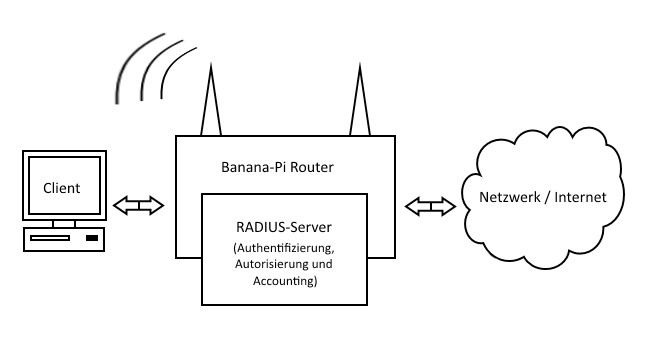
\includegraphics[width=\textwidth]{pictures/Tom/Radius}
\caption{Radius Funktionsweise}
\end{figure}
Anhand der obenstehenden Abbildung lässt sich gut erkennen wie der Aufbau ist. Der Client
(Smartphone, PC, etc.) kann sich wahlweise per WLAN oder LAN mit dem Banana-Pi Router
verbinden, dabei sendet er eine Authentifizierungsanfrage an diesen, welche der Router an den
Radius-Server, welcher auf dem Banana-Pi läuft, weiterleitet. Dieser verarbeitet nun die Anfrage
indem er, je nach Konfiguration, in unserem Fall über eine SQL-Datenbank überprüft ob der Client
berechtigt ist dem Netzwerk beizutreten. Zusätzlich kann diese Verbindung dann auch limitiert
werden (Volumen-Limit, Bandbreiten-Drosselung, beschränkter Zugriff auf Subnetze/VLANs).
\newpage

\subsection{FreeRADIUS}
FreeRADIUS ist wie der Name schon vermuten lässt eine freie und kostenlose Implementierung des
RADIUS-Protokolls und unter der GNU General Public License, version 2 lizenziert. Es ist laut
eigenen Angaben der weltweit am meisten eingesetzte RADIUS-Server und wird von den meisten
Internetdienstanbietern (Providern) sowie den 500 umsatzstärksten Unternehmen der Welt
benutzt. \cite{rad2}\\
Es findet außerdem auch in der Hochschule sowie im akademischen Forschungsnetzwerk Eduroam
Einsatz. Es unterstützt den meistverbreiteten Authentifizierungsstandard EAP, auf deutsch etwa„Erweiterbares Authentifizierungsprotokoll“ \cite{rad3}
, der ca. 40 verschiedene Verfahren anbietet, welche
heutzutage unter anderem in den Sicherheitsimplementationen WPA und WPA2 Verwendung
finden.\\
~\\
Installation:\\
FreeRADIUS ist auch in den offiziellen Paket-Quellen von Debian enthalten und kann somit ganz
einfach über den Debian-Paketmanager apt-get installiert werden. Als erstes stellen wir sicher dass
das System up-to-date ist und die aktuellen Paketquellen besitzt. \cite{rad4}
\begin{lstlisting}
sudo apt-get update
sudo apt-get upgrade
sudo apt-get freeradius freeradius-utils freeradius-mysql mysql-server
\end{lstlisting}
Bei der Installation des MySQL-Servers wird man gebeten das Passwort für den Root-User zu
setzen und zu bestätigen (in unserem Fall ist dies bananapi). Im nächsten Schritt wird eine
Datenbank für RADIUS angelegt.
\begin{lstlisting}
ql -uroot -p
\end{lstlisting}
\begin{lstlisting}
CREATE DATABASE radius;
GRANT ALL PRIVILEGES ON radius.* TO root@localhost IDENTIFIED BY "bananapi";
flush privileges;
exit
\end{lstlisting}
Danach noch die SQL Schemas in die Datenbank laden: \cite{rad5}
\begin{lstlisting}
mysql -uroot -p radius < /etc/freeradius/sql/main/mysql/schema.sql
mysql -uroot -p radius < /etc/freeradius/sql/main/mysql/setup.sql
\end{lstlisting}
Zukünftig können nun Benutzer mit folgendem MySQL-Befehl angelegt werden:
\begin{lstlisting}
insert into radcheck (username,attribute,op,value) values("USERNAME", "Cleartext-Password", ":=", "PASSWORD");
\end{lstlisting}
Nun muss RADIUS dafür konfiguriert werden, das SQL-Modul zu benutzen, dafür editiert man die
Datei /etc/freeradius/sql.conf und trägt im Bereich \#Connection info die korrekten Login-Daten ein.
Desweiteren muss man in der Datei radius.conf die Zeile \$INCLUDE sql.conf, sowie in der Datei
/etc/freeradius/sites-available/default zwei mal sql in den Sektionen authorize { und accounting
{ ein kommentieren.\\
~\\
Testen:\\
Um die Konfiguration zu überprüfen kann der RADIUS-Server im Debugging-Modus gestartet
werden. Dazu sollte der RADIUS-Dienst erst beendet werden:
\begin{lstlisting}
service freeradius stop
freeradius -X
\end{lstlisting}
Danach kann in einem zweiten Terminal (oder ggf. mit Terminal-Multiplexer) das Programm radtest
verwendet werden um Authentifizierungsanfragen an den RADIUS-Server zu senden: \cite{rad6}
\begin{lstlisting}
radtest USERNAME PASSWORD 127.0.0.1 0 mysecret
\end{lstlisting}
Eine typische Ausgabe einer erfolgreichen Anfrage sollte wie folgt aussehen:
\begin{figure}[ht]                    
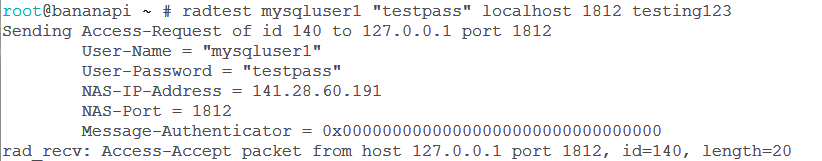
\includegraphics[width=\textwidth]{pictures/Tom/Radius2}
\caption{Radius Test}
\end{figure}














